\documentclass[12pt]{jreport}
\usepackage{comment}
\usepackage{./sty/eclepsf}
\usepackage{tascmac}
\usepackage{tabularx}
\usepackage{listliketab}
\usepackage[longnamesfirst]{natbib}
\usepackage[dvipdfmx]{graphics}
\usepackage[dvipdfmx]{graphicx}
\usepackage[dvipdfmx]{color}
\usepackage{subfigure}
\usepackage{alltt}
\usepackage{here}
\usepackage{afterpage}
\usepackage{./sty/ncodeline}
%\usepackage[dvipdfmx, colorlinks, breaklinks,%
\usepackage[dvipdfmx, breaklinks,%
bookmarks=true, bookmarksnumbered=true,%
bookmarkstype=toc, bookmarksopen=true,bookmarksopenlevel=3,%
pdftitle={RG},%
]{hyperref}
\usepackage{bookmark}

\AtBeginDvi{\special{pdf:tounicode EUC-UCS2}}

\usepackage{fancyhdr}

\usepackage{./sty/doxygenorig}

\usepackage{indentfirst}
\usepackage{url}
\usepackage{listings,./sty/jlisting}

\def\lstlistingname{プログラム}

\lstset{%
 language={C++},
 %backgroundcolor={\color[gray]{.85}},%
 basicstyle={\small\ttfamily},%
 identifierstyle={\small},%
 commentstyle={\small\itshape},%
 keywordstyle={\small\bfseries},%
 ndkeywordstyle={\small\ttfamily},%
 stringstyle={\small\ttfamily},
 frame={tb},
 framesep=1zw,
 breaklines=true,
 numbers=left,%
 xrightmargin=0zw,%
 xleftmargin=1.5zw,%
 numberstyle={\scriptsize},%
 stepnumber=1,
 numbersep=1zw,%
 lineskip=-0.5ex%
}

\usepackage{amssymb}
%\usepackage{supertabular,multirow}

\usepackage{array}
\newcolumntype{M}[1]{>{\centering\arraybackslash}m{#1}}

% A4  size: 297mm*210mm %1pt = 0.35mm
\setlength{\topmargin}{-3.4mm} % 10pt 25.4mm - 3.4mm = 22mm
\setlength{\oddsidemargin}{-0.4mm} % 25.4mm - 0.4mm = 25mm
\setlength{\evensidemargin}{-0.4mm} % 25.4mm - 0.4mm = 25mm
\setlength{\textheight}{231mm} % 660pt % original is 225.75mm 645pt
\setlength{\textwidth}{160mm} % 457pt

\renewcommand{\topfraction}{.99}
\renewcommand{\textfraction}{.0}
\renewcommand{\floatpagefraction}{.99}
\renewcommand{\bibname}{参考文献}


\pagestyle{fancy}
\lhead[]{}

\makeatletter
\def\chaptermark#1{\markboth {\ifnum \c@secnumdepth>\m@ne
\@chapapp\ \thechapter \@chappos\ \fi #1}{}}
\makeatother

% タイトル
\def\title{QRコードを用いたナビゲーションシステムの開発}
% 英語タイトル
\def\etitle{Development of navigation system with QR code}
% 著者(日本語)
\def\author{井手田悠希}
% 著者(英語)
\def\eauthor{Yuki Ideta}
% 学部・研究科
\def\dept{慶應義塾大学大学院 環境情報学部環境情報学科}
% 学部・研究科(英語)
\def\edept{Keio University Bachelor of Arts in Environment and Information Studies}

\begin{document}

\pagenumbering{roman}
\begin{titlepage}
  \begin{center}
    \begin{large}
      卒業論文   20019年度 (令和元年) \\
      \vspace{24pt}
      \title   
      \end{large}
  \end{center}
  \vspace{40em}
  \begin{flushright}
    \large \dept\\
    \author 
  \end{flushright}
\end{titlepage}

\thispagestyle{empty}


卒業論文要旨 - 2019年度 (令和元年度)
\begin{center}
\begin{large}
\begin{tabular}{|M{0.97\linewidth}|}
    \hline
      \title \\
    \hline
\end{tabular}
\end{large}
\end{center}
~ \\
現在UAVの自律飛行手法の多くはGPSでの誘導が多く、GPSが利用できない環境下ではLIDARやステレオカメラ、RGBDカメラなど何かしらの測量センサを積載し、それらの情報を基に飛行経路計算や障害物回避を行っている。  
GPSが利用できない環境とは橋の下や倉庫等の屋内など遮蔽物がある環境が挙げられる。  
~ \\
キーワード:\\
\underline{1. MAV},
\underline{2. 自己位置推定},
\underline{3. SLAM},
\underline{4. QRコード}
\begin{flushright}
\dept \\
\author
\end{flushright}

\thispagestyle{plain}
\clearpage

Abstract of Bachelor's Thesis - Academic Year 2019 - 2020
\begin{center}
\begin{large}
\begin{tabular}{|p{0.97\linewidth}|}
    \hline
      \etitle \\
    \hline
\end{tabular}
\end{large}
\end{center}

~ \\
There are 2 ways which realize automate item management system in the warehouse.  
The first way is using an automated rack or using robots to move a rack.
The second way is using patrol robots without any warehouse reform.  
This research focuses on the robot which is used in a second way.
We use a drone as a robot because the drone has many degrees of freedom.  
It is important that is route information and managed by software mainly.
However, It is verbose a little for patrol in the warehouse that already exists methods.
Thus, this research targeted the route control system and developed a stateless route control system.
In this system, we use QRCode to develop a stateless route control system and 
~ \\
Keywords : \\
\underline{1. Drone},
\underline{2. Navigation System},
\underline{3. WareHouse},
\underline{4. QRCode},
\begin{flushright}
\edept \\
\eauthor
\end{flushright}

\thispagestyle{plain}
\clearpage

\tableofcontents\thispagestyle{plain} %目次
\clearpage
\listoffigures\thispagestyle{plain} %図目次
\clearpage
\listoftables\thispagestyle{plain} %表目次
\clearpage

\pagenumbering{arabic}
\chapter{結論}
\label{conclusion}

本章では,本研究のまとめと今後の課題を示す.

\section{本研究のまとめ}
本研究で行った評価はあくまで今回利用した機材における性能評価に過ぎず,
実際にシステムとして実運用が可能かどうかは改めて実運用時の機材や環境での評価が必要であると考えられる.
今回利用した機材ではその仕様上20cm以下の細かい制御が出来ず,
位置補正にかかる時間はこの制御分解能にも大きく依存すると考えられるからである.
一方で,今回利用した機材は非常に簡易的な機材であるにも関わらず,
今回倉庫を想定して用意された棚では実用可能な精度で飛行する事が確認できた.
これらより本システムは倉庫の巡回タスクにおいては有効な手段である事を示した.
但し,利用する機材によって巡回速度や安定度は大きく左右する為,他の選択肢との比較を充分に行った上で採用する事が望ましい.


\section{本研究の課題}
\subsection{攻撃耐性}
本システム実際に使う上では間違って他のQRコードを認識してしまったり,
悪意ある人間によってQRコードがすり替えられていないかの検証システムが必要になってくる.
その場合にはjwtなどの方式でQRコード内のデータに署名をする.という事で対応できるが,
悪意ある人間がその環境に存在した場合QRコードの場所が置き換えられる可能性や複製されてしまうと言う可能性は残る.

\subsection{拡張性}
QRコードをLEDパネルで表示する方法\cite{led_qr}も考案されている為この方法を用いてQRコードを容易に変更・配置の記録をする事も可能になる.
どこにどのような内容のQRコードが配置されているかはシステム全体として保持しておきたい情報でもあり,LEDパネルでQRコードを表示する手法は本研究との親和性が非常に高いと考えられる.
また,この方法であれば動的にQRコードを変化させる事が可能であり,張り替えられたり複製されてしまう事への対策にもなり得る.
一方で本システムは経路情報の管理をシステムの外に出す事で制御システム自体の簡略化を図った物である事を考慮すると再び経路情報の管理用システムが必要となる点で本来の目的に反してしまう.
しかし制御システムから環境地図作成と専用機材を用意せず倉庫の巡回タスクを実施できるという点にメリットがある環境であれば検討の余地が充分にあると考えられる.

\subsection{精度向上}



%%% Local Variables:
%%% mode: japanese-latex
%%% TeX-master: "../thesis"
%%% End:

\chapter{結論}
\label{conclusion}

本章では,本研究のまとめと今後の課題を示す.

\section{本研究のまとめ}
本研究で行った評価はあくまで今回利用した機材における性能評価に過ぎず,
実際にシステムとして実運用が可能かどうかは改めて実運用時の機材や環境での評価が必要であると考えられる.
今回利用した機材ではその仕様上20cm以下の細かい制御が出来ず,
位置補正にかかる時間はこの制御分解能にも大きく依存すると考えられるからである.
一方で,今回利用した機材は非常に簡易的な機材であるにも関わらず,
今回倉庫を想定して用意された棚では実用可能な精度で飛行する事が確認できた.
これらより本システムは倉庫の巡回タスクにおいては有効な手段である事を示した.
但し,利用する機材によって巡回速度や安定度は大きく左右する為,他の選択肢との比較を充分に行った上で採用する事が望ましい.


\section{本研究の課題}
\subsection{攻撃耐性}
本システム実際に使う上では間違って他のQRコードを認識してしまったり,
悪意ある人間によってQRコードがすり替えられていないかの検証システムが必要になってくる.
その場合にはjwtなどの方式でQRコード内のデータに署名をする.という事で対応できるが,
悪意ある人間がその環境に存在した場合QRコードの場所が置き換えられる可能性や複製されてしまうと言う可能性は残る.

\subsection{拡張性}
QRコードをLEDパネルで表示する方法\cite{led_qr}も考案されている為この方法を用いてQRコードを容易に変更・配置の記録をする事も可能になる.
どこにどのような内容のQRコードが配置されているかはシステム全体として保持しておきたい情報でもあり,LEDパネルでQRコードを表示する手法は本研究との親和性が非常に高いと考えられる.
また,この方法であれば動的にQRコードを変化させる事が可能であり,張り替えられたり複製されてしまう事への対策にもなり得る.
一方で本システムは経路情報の管理をシステムの外に出す事で制御システム自体の簡略化を図った物である事を考慮すると再び経路情報の管理用システムが必要となる点で本来の目的に反してしまう.
しかし制御システムから環境地図作成と専用機材を用意せず倉庫の巡回タスクを実施できるという点にメリットがある環境であれば検討の余地が充分にあると考えられる.

\subsection{精度向上}



%%% Local Variables:
%%% mode: japanese-latex
%%% TeX-master: "../thesis"
%%% End:

\chapter{本研究における問題定義}
\label{issue}
カメラが搭載されている機体で、移動制御が行えるという事を条件にした自律制御を目的とする。
また、本手法はカメラ映像と移動制御が自由に行える機体であればどのような機体であっても利用できることを目指す。

また、GPSが利用できない倉庫等の屋内での自己位置推定を行い、安定した自律飛行をできるようにする事を目的としている。



%%% Local Variables:
%%% mode: japanese-latex
%%% TeX-master: "./thesis"
%%% End:

\chapter{提案手法}
\label{proposed}

本章では提案手法について述べる.

\section{概要}
基本の構成は以前作成した飛行モデルと変わらず、フラフープ検出部分をQRコードに変更したモデルで第一段階の実験を行う。



%%% Local Variables:
%%% mode: japanese-latex
%%% TeX-master: "../bthesis"
%%% End:

\chapter{実装}
\label{implementation}

本章では提案手法の実装について述べる.

\section{概要}
\begin{figure}[htbp]
  \begin{center}
    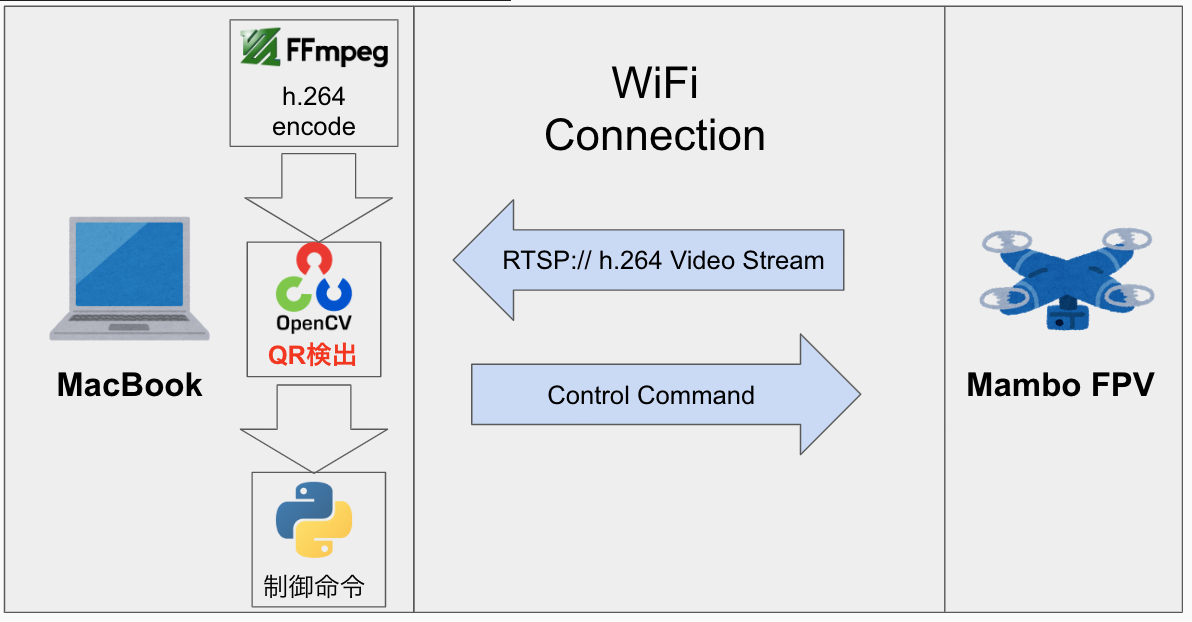
\includegraphics[clip,width=7.0cm]{img/sys-struct.png}
    \caption{構成図}
    \label{fig:struct}
  \end{center}
\end{figure}



%%% Local Variables:
%%% mode: japanese-latex
%%% TeX-master: "../bthesis"
%%% End:

\chapter{評価}
\label{evaluation}
本章では,提案システムの評価について述べる.

評価方法としては段階をいくつかに分け、段階に応じた評価を行う。
まず第一段階は各地点同士の距離をどこまで離しても飛行可能かを評価する。
QRコード同士の距離が離れれば離れるほどマーカーの未認識区間が広くなり、自己位置推定が難しくなる。
そのため、QRコードでの経路制御の限界距離をここで記録し、距離とコース通りの飛行の成功率を計測する。
ここでの飛行の成功、不成功は以下のように定義する。

「任意のQRコードAの正面からスタートし、次の地点Bへ到達し、QRコードを5秒以上フレームインし続ける事が出来るか。」

という条件を以って成功、不成功を定義する。

上記の評価に加えて、安定して地点間の移動が可能になった場合に次の段階に入る。
次の段階では既存の他のシステムとの比較を行う。
周回コースを用意し、同じコースを飛行する上でQRコードを用いた自己位置推定システムとVO(Visual Odometry)での自己位置推定と比較する。
精度の比較はコースの周回速度と成功率で比較する。
成功率は上記での定義を同様に用いる物とする。

\section{評価内容}



%%% Local Variables:
%%% mode: japanese-latex
%%% TeX-master: "./thesis"
%%% End:

\chapter{関連研究}
\label{related_works}

基本的にドローンが自律飛行を行う際に必要とされる処理がいくつかある.そのうちの2つが自己位置推定と姿勢推定である.
自己位置推定とは,ドローンが飛行している空間の中で自分がどの位置にいるのかを認識する事である.姿勢推定とは自分が水平方向に対してどの程度傾いているのか,鉛直方向に対してどの程度回転しているかといった事を認識することある.

\section{Nanomap}
これらを行なっている関連研究としてNanomap\cite{Nanomap}という飛行モデルがある.においては2D-LIDARを用いた飛行経路探索手法が取られており,取得した点群データを過去数フレーム分を記憶しておき,過去の数フレーム分のデータと現在のフレームとの点群の変量によっておおよその障害物の位置を認識している.こちらの手法では,物体を正確に捉えることは放棄し,不確実な部分を物体の存在している可能性のある範囲として捉えている.視野にある物体のある可能性も含めて1番物体が少ない方向を飛行経路として選定し,飛行している.

\section{Octomap}
他に,ドローンに限らずロボット工学全般で利用されてきたOctomap\cite{Octomap}がある.
こちらもNanomapと同様にLIDARを用いて周辺の環境情報を扱うものであるが,こちらはLIDARを用いて実際に周囲を点群からモデリングして周辺状況を把握する.

Octomapではモデリングする際に近い点群同士を同じ物体としてまとめ1つのブロックにするということを繰り返し,樹構造的にブロックを生成する為,生成後のデータは繰り返す回数等のパラメータによっては小さく圧縮することもできる.
\begin{figure}[htbp]
  \begin{center}
    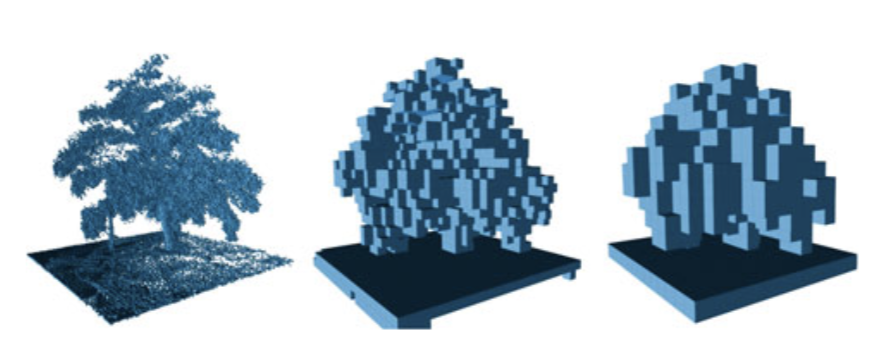
\includegraphics[clip,width=7.0cm]{img/octomap.png}
    \caption{圧縮率の違いによる生成物の違い}
    \label{fig:hamu}
  \end{center}
\end{figure}
しかし,実際に点群からモデルを生成するとなるとその計算量は非常に多く,高性能な小型コンピュータが現れている現在においても処理負荷が大きく,特にドローンにおいては積載量に制限がかかりやすい為扱いにくいものとなっている.


\section{実用性を備えた手のひらサイズ・完全オンボード処理 UAV}
また,これらのようにLIDARを使用せず,CMOSセンサーのみで自律飛行を行なっている例もある.

実用性を備えた手のひらサイズ・完全オンボード処理 UAV のための 3 次元自己位置推定手法の提案と全自動飛行の実現\cite{SfMDrone}では自己位置推定で使用するセンサーはCMOSセンサーを利用した自律飛行を実現している.
CMOSセンサーからの映像をFPGAにストリームしてFAST\cite{FAST}による特徴点抽出処理を行い,その結果をBrief\cite{Brief}を用いて表現し,MCUに流し込み処理している.この研究での目的は外部処理系に依存せず,ドローン上で全て完結する自律飛行可能な小型ドローンの開発で,限定条件下(新聞紙を敷き詰めた床面)の上で飛行させ,特徴点を十分に検出できるようにした上で,飛行させ想定通りの飛行を実現している.

\section{DeepDrone}
他に今回の研究のベース物としてDeepDrone\cite{DeepDrone}が挙げられる.こちらではドローンレースを自律飛行で行う為に自律飛行モデルを提案している.ドローンレースとは基本的にゲートを順に潜りながら飛行することが条件となっているドローン競技である.このゲートをRGBカメラで撮影した映像を推定モデルに対し,200*300の画像を所与として$\lbrace \vec{x}, v \rbrace$,を推定結果として得る.$\lbrace \vec{x}$は$\vec{x} \in [-1,1]^2$と定義され正規化された入力画像の中にある目標とするゲートへの方向を表していおり, $v \in [0,1]$ は飛行速度を正規化して表している. 

DeepDroneでは訓練にシミュレータでのデータと現実世界でのデータを使っている.両者とも理想とする軌道とのズレを計算しそのズレを損失関数に入力し学習を進めていく.
\begin{figure}[htbp]
  \begin{center}
    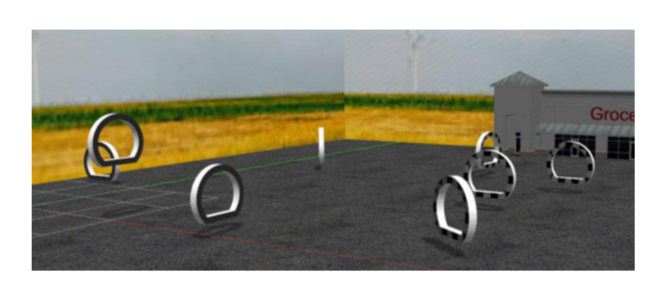
\includegraphics[clip,width=7.0cm]{img/deep-simu.png}
    \caption{シミュレータ上のゲート}
    \label{fig:gate}
  \end{center}
\end{figure}
シミュレータ上では直接理想とする軌道とのズレを取得し,実空間では実際に手動で実際のコース上を運び,ゲートを通過させるなどしてデータを収集していた.

\section{TDOAを用いたUAVの自己位置推定}
他に屋内でドローンの位置測位を行っている例としてScalable and Precise Multi-UAV Indoor Navigation\cite{TDOA-UWB}が挙げられる。これはTDOA-UWBという方式を用いたものである。TDOA(Time Differences of Arrival)とは電波を用いた位置推定手法でありTOA(Time of Arrival)とよく比較される。Time of Arrivalでは電波を発信する送信機と位置推定を行う受信機との構成で行われる。送信機と受信機で時刻同期を行った上で、各送信機からの伝播時間を計測。この電波時間から距離を計算し、複数の送信機を用いると位置推定を行う事が出来る。

一方でTDOAでは時刻同期の必要はなく、送信されてくる電波の時間差を用いて位置推定を行う。
今回挙げているこの例ではTDOAによる位置測位を行うのにUWBを電波として用いている。


\section{TERMプロジェクトでの成果}
他に関連研究として自身の以前作成した飛行モデルをここで紹介したい。
前回作成したモデルは黄色のフラフープをターゲットとしてフラフープをハフ変換とカラーフィルターを利用して検出し、そのフラフープを通過するというものである。実際のシステム概略図は以下のようになっている。

\begin{figure}[htbp]
  \begin{center}
    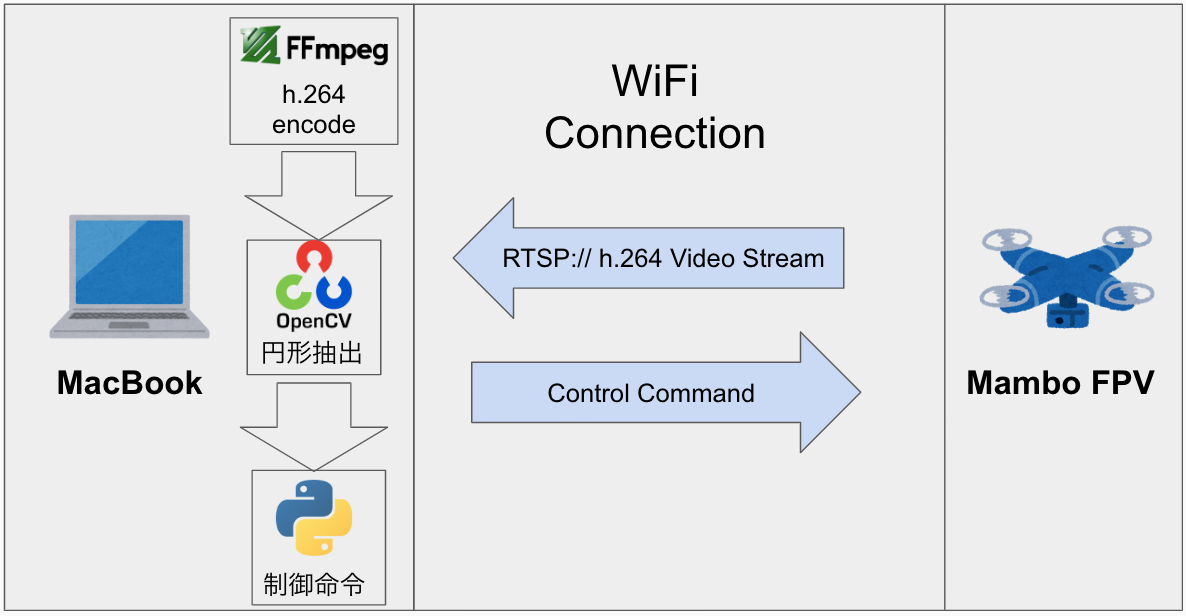
\includegraphics[clip,width=7.0cm]{img/term-system.png}
    \caption{フラフープ通過飛行モデル}
    \label{fig:gate}
  \end{center}
\end{figure}

この飛行モデルでは歪み補正や傾きを考慮しておらず、地図情報を生成してもいない為一度フラフープがフレームアウトしたり、フラフープの正面方向に対して30°以上角度がついてしまうと通過率が著しく落ちる事がわかっている。



%%% Local Variables:
%%% mode: japanese-latex
%%% TeX-master: "./thesis"
%%% End:

\chapter{結論}
\label{conclusion}

本章では,本研究のまとめと今後の課題を示す.

\section{本研究のまとめ}
今回のこのシステム実際に使う上では間違って他のQRコードを認識してしまったり、悪意ある人間によってQRコードがすり替えられていないかの検証システムが必要になってくる。
その場合にはjwtなどの方式でQRコード内のデータに署名をする。という事で対応できるが、QRコードの場所が置き換えられてしまう、複製されてしまう。という問題は残る。

これらの事より本システムは悪意のある人間がいない環境での利用が制約として加わることになると考えられる。

\section{本研究の課題}

%%% Local Variables:
%%% mode: japanese-latex
%%% TeX-master: "../thesis"
%%% End:

\appendix
\chapter{付録}

\section{付録内容}
周回時各地点での位置補正に要した秒数のデータ\ref{log_data}
\begin{lstlisting}[caption=log\_data.csv,label=log_data]
    index,start_time,end_time,diff
    1,1580193930.29,1580193976.28,-45.9868371487
    2,1580193990.3,1580193994.3,-4.00511908531
    3,1580194009.33,1580194013.32,-3.98436999321
    4,1580194028.36,1580194032.34,-3.97335982323
    5,1580194035.4,1580194039.46,-4.06102204323
    6,1580194052.82,1580194068.8,-15.9791119099
    7,1580194083.81,1580194087.82,-4.00577402115
    8,1580194102.83,1580194118.84,-16.0141539574
    9,1580194132.9,1580194144.87,-11.9710979462
    1,1580196624.09,1580196667.6,-43.5060019493
    2,1580196681.69,1580196685.71,-4.02595710754
    3,1580196701.1,1580196721.41,-20.3125030994
    4,1580196736.47,1580196740.43,-3.9612288475
    5,1580196753.45,1580196757.45,-4.00381112099
    6,1580196772.49,1580196776.47,-3.97698187828
    7,1580196791.52,1580196795.49,-3.97074103355
    8,1580196809.54,1580196813.51,-3.97161698341
    9,1580196820.23,1580196823.28,-3.04999995231
    1,1580198671.04,1580198714.29,-43.2508609295
    2,1580198728.31,1580198732.31,-4.00313401222
    3,1580198747.38,1580198751.33,-3.95450305939
    4,1580198766.39,1580198782.36,-15.9714820385
    5,1580198795.41,1580198799.38,-3.97379899025
    6,1580198814.42,1580198818.4,-3.97790408134
    7,1580198833.42,1580198837.42,-3.99298119545
    8,1580198851.44,1580198879.46,-28.0157217979
    9,1580198892.49,1580198896.47,-3.98590183258
    1,1580199262.13,1580199304.84,-42.7095551491
    2,1580199318.89,1580199339.25,-20.359513998
    3,1580199354.6,1580199358.56,-3.96238017082
    4,1580199373.89,1580199377.88,-3.99445414543
    5,1580199390.94,1580199403.26,-12.3130421638
    6,1580199418.3,1580199422.28,-3.97520399094
    7,1580199437.29,1580199441.3,-4.00463104248
    8,1580199455.35,1580199471.63,-16.2756249905
    9,1580199484.76,1580199505.0,-20.2366819382
    1,1580200356.27,1580200450.39,-94.1180570126
    2,1580200464.46,1580200468.41,-3.9505751133
    3,1580200483.44,1580200504.44,-21.0034091473
    4,1580200519.51,1580200523.46,-3.94975781441
    5,1580200536.52,1580200556.56,-20.0388579369
    6,1580200571.89,1580200591.89,-20.0021989346
    7,1580200606.94,1580200610.91,-3.96967601776
    8,1580200624.94,1580200628.93,-3.98880791664
    9,1580200641.97,1580200645.94,-3.97123003006
    1,1580201161.0,1580201187.53,-26.5303680897
    2,1580201201.89,1580201213.86,-11.9634230137
    3,1580201228.91,1580201244.89,-15.9810349941
    4,1580201259.92,1580201290.93,-31.0086560249
    5,1580201303.94,1580201344.98,-41.0400719643
    6,1580201360.04,1580201380.02,-19.974052906
    7,1580201395.07,1580201399.04,-3.96285891533
    8,1580201413.05,1580201438.38,-25.3258821964
    9,1580201451.45,1580201455.4,-3.94306898117
    1,1580202744.16,1580202809.66,-65.5057330132
    2,1580202823.73,1580202872.72,-48.9925370216
    3,1580202887.75,1580202899.75,-12.0069699287
    4,1580202914.78,1580202918.77,-3.99462604523
    5,1580202932.11,1580202936.09,-3.98409891129
    6,1580202951.16,1580202975.13,-23.9704370499
    7,1580202990.18,1580202994.15,-3.97114396095
    8,1580203008.22,1580203012.17,-3.95584893227
    9,1580203025.2,1580203029.19,-3.98650503159
    1,1580204346.96,1580204422.06,-75.0941159725
    2,1580204436.1,1580204440.07,-3.97245383263
    3,1580204455.13,1580204475.1,-19.9742369652
    4,1580204490.15,1580204494.12,-3.97111201286
    5,1580204507.18,1580204531.16,-23.9756538868
    6,1580204546.19,1580204550.18,-3.9876408577
    7,1580204565.24,1580204577.2,-11.9651100636
    8,1580204591.27,1580204595.22,-3.94821619987
    9,1580204608.29,1580204612.24,-3.94957995415
    1,1580208884.14,1580208939.61,-55.4682879448
    2,1580208953.66,1580208957.63,-3.9718708992
    3,1580208972.67,1580209012.05,-39.3805930614
    4,1580209027.07,1580209031.07,-4.00029397011
    5,1580209044.09,1580209064.1,-20.0068509579
    6,1580209079.15,1580209083.12,-3.97090888023
    7,1580209098.15,1580209110.15,-11.9959571362
    8,1580209124.18,1580209128.17,-3.98279809952
    9,1580209141.19,1580209153.19,-11.999601841
    1,1580210529.13,1580210583.77,-54.6374969482
    2,1580210598.11,1580210602.09,-3.97895812988
    3,1580210617.11,1580210653.44,-36.3331010342
    4,1580210668.5,1580210672.46,-3.96202206612
    5,1580210685.52,1580210745.52,-60.0027010441
    6,1580210760.61,1580210788.6,-27.9818811417
    7,1580210803.65,1580210807.62,-3.96309781075
    8,1580210821.63,1580210825.71,-4.08048391342
    9,1580210839.02,1580210843.02,-4.00416183472
\end{lstlisting}

今回実験に使用したスクリプト\ref{controller}
\begin{lstlisting}[caption=controller.py,label=controller]
#!/usr/bin/env python
# -*- coding:utf-8 -*-
import threading
import time
import numpy as np
import json

import cv2


class Controller(object):
    def __init__(self, drone):
        # init objs
        self.drone = drone
        self.thread = None
        self.stopEvent = None
        self.QR_SIZE = 14.2
        self.UNIT_SIZE = 2.4
        self.RAD_UNIT = 180/3.14
        self.SPEED = 10
        self.Z_SPACE = 85
        self.permit_noise = 10
        self.COMMAND_WAIT_BUFFER = 3
        self.objp = np.array([
            [[0, 0, 0]],
            [[self.QR_SIZE/self.UNIT_SIZE, 0, 0]],
            [[self.QR_SIZE/self.UNIT_SIZE, self.QR_SIZE/self.UNIT_SIZE, 0]],
            [[0, self.QR_SIZE/self.UNIT_SIZE, 0]]
        ], dtype="float32")
        self.axis = np.float32([
            [self.QR_SIZE/self.UNIT_SIZE, 0, 0],
            [0, self.QR_SIZE/self.UNIT_SIZE, 0],
            [0, 0, -1 * self.QR_SIZE/self.UNIT_SIZE]
        ]).reshape(-1, 3)
        self.mtx = np.load("tello_mtx.npy")
        self.dist = np.load("tello_dist.npy")
        self.count = 1
        self.fourcc = cv2.VideoWriter_fourcc(*'XVID')
        self.out = cv2.VideoWriter('default.avi',
                                   self.fourcc, 20.0, (960, 720))
        self.is_moving = False
        self.is_standby = False
        self.target_pos = {
            'x': 0,
            'y': 0,
            'z': 0,
            'r': 0
        }
        self.drone_rotate_list = []
        self.drone_pos_list = []
        self.drone_pos = {
            'x': 0,
            'y': 0,
            'z': 0,
            'r': 0
        }
        self.log_data = {}

        # init methods
        self.stopEvent = threading.Event()
        self.thread = threading.Thread(target=self.video_loop)
        self.thread.start()
        self.send_command_thread = \
            threading.Thread(target=self._sending_command)
        self.send_command_thread.start()
        self.drone.set_speed(self.SPEED)
        self.drone.takeoff()
        time.sleep(7)
        self.main()

    def __del__(self):
        self.drone.land()
        self.out.release()
        time.sleep(3)
        self.stopEvent.set()

    def video_loop(self):
        try:
            time.sleep(0.5)
            while not self.stopEvent.is_set():
                frame = self.drone.read()
                if frame is None or frame.size == 0:
                    continue
                self.pnp_qr(frame)
        except(KeyboardInterrupt, SystemExit):
            self.stopEvent.set()
            print('exit video loop')

    def _sending_command(self):
        while not self.stopEvent.is_set():
            self.drone.send_command('command')
            print('battery: ', self.drone.get_battery())
            time.sleep(5)

    def draw(self, img, corners, imgpts):
        try:
            corner = tuple(corners[0].ravel())
            img = cv2.line(img, corner, tuple(
                imgpts[0].ravel()), (255, 0, 0), 5)
            img = cv2.line(img, corner, tuple(
                imgpts[1].ravel()), (0, 255, 0), 5)
            img = cv2.line(img, corner, tuple(
                imgpts[2].ravel()), (0, 0, 255), 5)
            return img
        except Exception:
            return img

    def _qr_validator(self, data):
        x = data['x'] if 'x' in data else 0
        y = data['y'] if 'y' in data else 0
        z = data['z'] if 'z' in data else 0
        r = data['rotate'] if 'rotate' in data else 0
        return {'x': x, 'y': y, 'z': z, 'r': r }

    def pnp_qr(self, frame):
        img = cv2.cvtColor(frame, cv2.COLOR_RGB2BGR)

        qr = cv2.QRCodeDetector()
        data, points, _ = qr.detectAndDecode(img)
        if data:
            self.qr_data = self._qr_validator(json.loads(data))
            _, origin_rvec, origin_tvec, inliers = cv2.solvePnPRansac(
                self.objp, points, self.mtx, self.dist)
            if not self.is_moving:
                self.target_pos = self.qr_data
                tvec = origin_tvec * self.UNIT_SIZE
                rvec = origin_rvec * self.RAD_UNIT
                self.drone_pos_list.append(tvec)
                self.drone_rotate_list.append(rvec)
                if len(self.drone_pos_list) > 20:
                    self.drone_pos_list.pop(0)
                    self.drone_rotate_list.pop(0)
                drone_avg_pos = np.mean(self.drone_pos_list, axis=(0))
                drone_avg_rotate = np.mean(self.drone_rotate_list, axis=(0))
                self.drone_pos = {
                    'x': drone_avg_pos[0],
                    'y': drone_avg_pos[1],
                    'z': drone_avg_pos[2],
                    'r': drone_avg_rotate[1]
                }
            imgpts, jac = cv2.projectPoints(
                self.axis, origin_rvec, origin_tvec, self.mtx, self.dist)
            img = self.draw(img, points, imgpts)

            cv2.imshow('img', img)
            cv2.waitKey(10)
        else:
            cv2.imshow('img', img)
            cv2.waitKey(10)
        if not self.count in self.log_data:
            self.log_data[self.count] = time.time()
        self.out.write(img)

    def close_to_qr(self):
        print('self pos: ', self.drone_pos)
        move_x_val = int(self.drone_pos["x"] - (self.QR_SIZE/2))
        move_y_val = int(self.drone_pos["y"] - (self.QR_SIZE/2))
        move_z_val = int(self.drone_pos["z"] - self.Z_SPACE)
        rotate_val = int(self.drone_pos["r"])
        move_data = {
            "x": move_x_val,
            "y": move_y_val,
            "z": move_z_val,
            "r": rotate_val
        }
        self._move(move_data)
        return

    def go_to_target(self):
        print('self pos: ', self.drone_pos)
        move_data = {
            "x": self.target_pos["x"],
            "y": -self.target_pos["y"],
            "z": self.target_pos["z"],
            "r": self.target_pos["r"]
        }
        self.count += 1
        self.log_data[self.count] = time.time()
        with open('log_data.csv',"a") as f:
            f.write(str(self.count/2)+","+str(self.log_data[self.count-1])+","+str(self.log_data[self.count])+","+str(self.log_data[self.count-1]-self.log_data[self.count])+"\n")
        self._move(move_data)
        self.count += 1
        self.target_pos = {
            'x': 0,
            'y': 0,
            'z': 0,
            'r': 0
        }
        return

    def _move(self, data):
        self.is_moving = True
        # move x
        if data["x"] >= 10:
            self.drone.move_right(data["x"])
            time.sleep(data["x"]/self.SPEED + self.COMMAND_WAIT_BUFFER)
            print('sleep x: ', data["x"]/self.SPEED +
                  self.COMMAND_WAIT_BUFFER)
        elif data["x"] <= -10:
            self.drone.move_left(-data["x"])
            time.sleep(-data["x"]/self.SPEED + self.COMMAND_WAIT_BUFFER)
            print('sleep x: ', -data["x"]/self.SPEED +
                  self.COMMAND_WAIT_BUFFER)
        # move y
        if data["y"] >= 10:
            self.drone.move_down(data["y"])
            time.sleep(data["y"]/self.SPEED + self.COMMAND_WAIT_BUFFER)
            print('sleep y: ', data["y"]/self.SPEED +
                  self.COMMAND_WAIT_BUFFER)
        elif data["y"] <= -10:
            self.drone.move_up(-data["y"])
            time.sleep(-data["y"]/self.SPEED + self.COMMAND_WAIT_BUFFER)
            print('sleep y: ', -data["y"]/self.SPEED +
                  self.COMMAND_WAIT_BUFFER)
        # move z
        if data["z"] >= 10:
            self.drone.move_forward(data["z"])
            time.sleep(data["z"]/self.SPEED + self.COMMAND_WAIT_BUFFER)
            print('sleep z: ', data["z"]/self.SPEED +
                  self.COMMAND_WAIT_BUFFER)
        elif data["z"] <= -10:
            self.drone.move_backward(-data["z"])
            time.sleep(-data["z"]/self.SPEED + self.COMMAND_WAIT_BUFFER)
            print('sleep z: ', -data["z"]/self.SPEED +
                  self.COMMAND_WAIT_BUFFER)
        # rotate r
        if data["r"] > 0:
            self.drone.rotate_cw(data["r"])
        else:
            self.drone.rotate_ccw(-data["r"])
        time.sleep(self.COMMAND_WAIT_BUFFER)
        # initialize values
        self.is_moving = False
        self.is_standby = False
        self.drone_pos_list = []
        self.drone_rotate_list = []
        return

    def check_standby(self):
        x_val = int(self.drone_pos["x"] - (self.QR_SIZE/2))
        y_val = int(self.drone_pos["y"] - (self.QR_SIZE/2))
        z_val = int(self.drone_pos["z"] - self.Z_SPACE)
        rotate_val = int(self.drone_pos["r"])
        self.is_standby = -self.permit_noise < x_val and self.permit_noise > x_val and \
            -self.permit_noise < y_val and self.permit_noise > y_val and \
            -self.permit_noise < z_val and self.permit_noise > z_val and \
            -self.permit_noise < rotate_val and self.permit_noise > rotate_val
        print('check: ', x_val, y_val, z_val, rotate_val)
        print('is_standby: ', self.is_standby)


    def main(self):
        # main thread
        # main thread is sending command and waiting for keyboardInterrupt
        try:
            while True:
                self.close_to_qr()
                self.check_standby()
                time.sleep(1)
                if self.is_standby:
                    self.go_to_target()
                if self.count == 100:
                    break
        except(KeyboardInterrupt, SystemExit):
            self.__del__()
            print("exit")
        self.__del__()
\end{lstlisting}
\chapter*{謝辞}
\addcontentsline{toc}{chapter}{謝辞}
\label{thanks}





%%% Local Variables:
%%% mode: japanese-latex
%%% TeX-master: "../yummy_bthesis"
%%% End:


\renewcommand{\thechapter}{\Alph{chapter}}
\setcounter{chapter}{0}
\vspace{-5mm}


\begin{thebibliography}{99}
%\bibitem{a}
\bibitem{Nanomap}
\texttt{Peter R. Florence1, John Carter1, Jake Ware1, Russ Tedrake1, NanoMap: Fast, Uncertainty-Aware Proximity Queries with Lazy Search over Local 3D Data}

\bibitem{Octomap}
\texttt{A. Hornung, K. M. Wurm, M. Bennewitz, C. Stachniss, and W. Burgard, “Octomap: An efficient probabilistic 3d mapping framework based on octrees,” Auton. Robots, vol. 34, no. 3, pp. 189–206, Apr. 2013. [Online]. Available: http://dx.doi.org/10.1007/ s10514- 012- 9321- 0}

\bibitem{Voxblox}
\texttt{H. Oleynikova, Z. Taylor, M. Fehr, J. Nieto, and R. Siegwart, “Voxblox: Building 3d signed distance fields for planning,” arXiv preprint arXiv:1611.03631, 2016.}

\bibitem{SfMDrone}
\texttt{此村 領, 堀 浩1, 実用性を備えた手のひらサイズ・完全オンボード処理 UAV のための 3 次元自己位置推定手法の提案と全自動飛行の実現, 東京大学工学系研究科航空宇宙工学専攻}

\bibitem{FAST}
\texttt{E. Rosten, R. Porter, and T. Drummond. “Faster and better: A machine learning approach to corner detection.” IEEE Trans. Pattern Analysis and Machine Intelligence, 32:105-119, 2010.}

\bibitem{Brief}
\texttt{M. Calonder, V. Lepetit, C. Strecha, and P. Fua. “Brief: Binary robust independent elementary features.” In European Conference on Computer Vi- sion, 2010.}

\bibitem{DeepDrone}
\texttt{Deepa Kaufmann, Antonio Loquercio, Rene Ranftl, Alexey Dosovitskiy, Vladlen Koltun, Davide Scaramuzza, Drone Racing: Learning Agile Flight in Dynamic Environments, University of Zurich and ETH Zurich Intel Labs}

\bibitem{Honda}
\texttt{横山 利夫,武田 政宣,藤田 進太郎,安井 裕司,Hondaの運転支援および自動運転の現状と今後,本田技術研究所四輪R&D センター 栃木県芳賀郡芳賀町下高根沢}

\end{thebibliography}
\thispagestyle{plain}%bibtex


\end{document}

%%% Local Variables:
%%% mode: japanese-latex
%%% TeX-master: t
%%% End:
